\section{示例程序}

\begin{frame}[fragile]\ft{\secname}
\lstinputlisting[language=c,numbers=left]{ch05/code/shoe1.c} 

\end{frame}


\begin{frame}[fragile]\ft{\secname}
\begin{lstlisting}[backgroundcolor=\color{red!10}]
$ gcc shoe1.c
$ ./a.out 
Shoe size (men's)   foot length
       9.0           10.56 inches
\end{lstlisting}
\end{frame}


\begin{frame}[fragile,allowframebreaks]\ft{\secname}
\lstinputlisting[language=c,frame=single,numbers=left]{ch05/code/shoe2.c} 
\end{frame}



\begin{frame}[fragile]\ft{\secname}
\begin{lstlisting}[backgroundcolor=\color{red!10}]
$ gcc shoe2.c
$ ./a.out 
Shoe size (men's)  foot length
      12.0           11.54 inches
      13.0           11.87 inches
      14.0           12.19 inches
      15.0           12.52 inches
      16.0           12.84 inches
      17.0           13.16 inches
      18.0           13.49 inches
If shoes fit, wear it.
\end{lstlisting}
\end{frame}


\begin{frame}[fragile]\ft{while循环}
\begin{lstlisting}[language=c,frame=single]
while (condition)
  statement
\end{lstlisting}

\begin{lstlisting}[language=c,frame=single]
while (condition)
{
  statements
}
\end{lstlisting}

\begin{lstlisting}[language=c,frame=single]
while (condition){
  statements
}
\end{lstlisting}


\end{frame}


\begin{frame}[fragile]\ft{while循环}
\begin{figure}
\centering
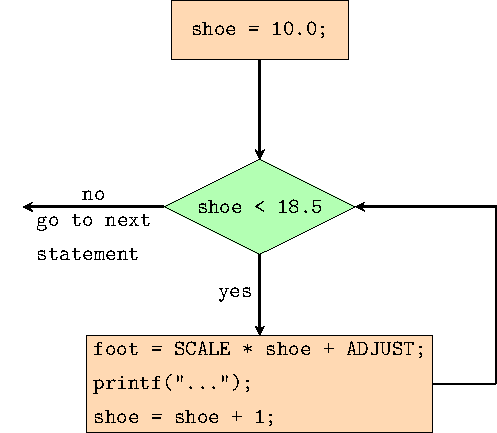
\includegraphics[width=3in]{ch05/images/while.pdf}
\end{figure}
\end{frame}
